\documentclass[11pt,a4paper]{article}

%biblioteci
\usepackage[romanian]{babel}  % bibliografia si cuprinsul sa fie in romana
% \usepackage{times} % times new roman
\usepackage{csquotes} % pt warning
\usepackage{lipsum}
\usepackage{indentfirst} % pentru ca si primul paragraf sa aiba alineat
\usepackage{graphicx}  % pentru inserare imagini
\usepackage{float} % pt asezare imagini in pagina
\usepackage{hyperref} % pt cuprins cu linkuri catre sectiuni
\usepackage{minted} % pt cod
\usepackage{algorithm}
\usepackage{algpseudocode}
\usepackage{amsmath}

\hypersetup{
    colorlinks,
    citecolor=black,
    filecolor=black,
    linkcolor=black,
    urlcolor=black
}

\usepackage{biblatex}

% format document(margin)
\usepackage[top=2.5cm, bottom=2.5cm, left=2.5cm, right=2.5cm]{geometry}
\linespread{1.06} % spatiu intre cuvinte
\setlength{\parskip}{8pt plus2pt minus2pt} % spatiu intre paragrafe

% widow and orphan lines
\widowpenalty 10000
\clubpenalty 10000

\newcommand{\eat}[1]{}
\newcommand{\HRule}{\rule{\linewidth}{0.5mm}}

%puncte si dupa fiecare sectiune in cuprins
\usepackage{tocloft}
\renewcommand{\cftsecleader}{\cftdotfill{\cftdotsep}}

% pentru bibliografie
% \usepackage{biblatex} % Imports biblatex package
% \addbibresource{refs.bib} % Import the bibliography file

% afiseaza mai frumos listele
\usepackage{enumitem} % ceva control asupra listelor/ enumerarilor
\setlist{nolistsep,noitemsep}

\setlength{\parskip}{2pt}  % spatiu intre paragrafe

\begin{document}

\begin{titlepage}
\begin{center}

% Top 

\includegraphics[width=0.55\textwidth]{resources/utcn_logo.jpg}~\\[2cm]

% Title
\HRule \\[0.4cm]
{ \LARGE
    \textbf{Probleme de cautare si agenti adversariali}\\[0.4cm]
    \emph{Inteligenta Artificiala}\\[0.4cm]
}
\HRule \\[1.5cm]

% Author
{ \large
    Autori: Oprisor Paul si Turda Sorin\\[0.1cm]
    Grupa: 30232\\[0.1cm]
}

\vfill
\textsc{\large Facultatea de Automatica\\si Calculatoare}\\[0.4cm]

% Bottom
{\large 3 Decembrie 2024}
    
\end{center}
\end{titlepage}
\tableofcontents % afiseaza cuprinsul
\section{Tutorial}  % titlu principal

\subsection{Subtitlu 1}  % subtitlu
\lipsum[1-2] % doar pentru exemplu, adauga textul ala in latina

\subsubsection{Subsubtitlu} % subtitlu la subtitlu
\par Born into the noble Crownguard family, along with his younger sister Lux, Garen knew from an early age that he would be expected to defend the throne of Demacia with his life. His father, Pieter, was a decorated military officer, while his aunt Tianna was Sword-Captain of the elite Dauntless Vanguard—and both were recognized and greatly respected by King Jarvan III. It was assumed that Garen would eventually come to serve the king’s son in the same manner.

\subsection{Tutorial elemente de baza}
\par O propozitie normala. Daca vrem sa adaugam text in \textbf{bold}, \textit{italic} sau \textbf{\textit{bold italic}}. \\ % cele doua backslash-uri sunt pentru a trece la un rand nou
Astfel se poate utiliza o \textbf{lista numerotata}:

% lista numerotata
\begin{enumerate}
    \item primul element
    \item al doilea element
    \item al treilea element
\end{enumerate}
Astfel se poate utiliza o \textbf{lista neumerotata}:

% lista neumerotata
\begin{itemize}
    \item primul element
    \item al doilea element
    \item al treilea element
\end{itemize}

\par Asa se adauga o \textbf{imagine}.
\begin{figure}[H]
    \centering  % centrare imagine
    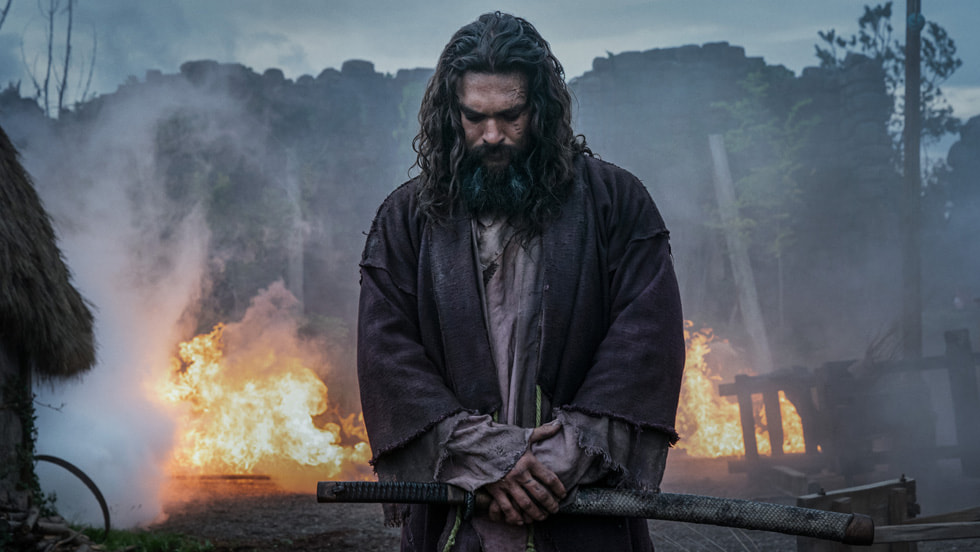
\includegraphics[scale=0.35]{resources/see_image.jpg}  % scale este factorul de scalare al imaginii originale
    \caption{Baba Voss}  % titlu imagine
    \label{fig:figura1} % label pentru referire
\end{figure}
% fig:figura1 este numele label-ului. Se putea folosi pur si simplu si "gigel", insa este o conventie ca label-urile
% figurilor sa fie de forma "fig:nume_figura"
Daca vrem sa referim imaginea \ref{fig:figura1} in text se procedeaza astfel.


\section{Uninformed search}
\subsection{Question 1 - Gasirea unui punct unde se afla mancare folosind Depth-First Search}
% definire cerinta
\par Gasirea unui punct unde se afla mancare folosind Depth First Search
\par \textbf{Depth-First Search} este un algoritm utilizat pentru explorarea grafurilor sau arborilor. Scopul acestuia este de a traversa toate nodurile unui graf, urmărind o cale cât mai adâncă înainte de a reveni și a explora căile neexplorate.
% prezentare algoritm/metoda

\begin{algorithm}
\caption{Iterative Depth-First Search (DFS)}
\begin{algorithmic}[1]
\Procedure{IterativeDFS}{$G, v$}
    \State Initialize an empty stack $S$
    \State Push $v$ onto $S$
    \State Mark $v$ as visited
    \While{$S$ is not empty}
        \State $u \gets$ \Call{Pop}{$S$}
        \For{each neighbor $w$ of $u$ in $G$}
            \If{$w$ is not visited}
                \State Push $w$ onto $S$
                \State Mark $w$ as visited
            \EndIf
        \EndFor
    \EndWhile
\EndProcedure
\end{algorithmic}
\end{algorithm}

% optional prezentare cod
% optional explicatii suplimentare cod

% comentarii/observatii asupra performantei/rezultatelor/complexitatii/algoritmului

\subsection{Question 2 - Breadth-first search}
\par \textbf{Breadth-first search} este un algoritm utilizat pentru traversarea și căutarea în grafuri sau arbori. Spre deosebire de DFS, BFS explorează nodurile pe niveluri, adică parcurge mai întâi toate nodurile aflate la o anumită distanță de nodul de start înainte de a trece la nodurile mai îndepărtate. BFS este implementat utilizând o coadă pentru a gestiona ordinea vizitării nodurilor.
% TODO: de completat
% + q3 din project 1

\begin{algorithm}
\caption{Breadth First Search (BFS)}
\begin{algorithmic}[1]
\Procedure{BFS}{$G, s$} \Comment{$G$ is the graph, $s$ is the starting node}
    \State Initialize an empty queue $Q$
    \State Enqueue $s$ into $Q$
    \State Mark $s$ as visited
    \While{$Q$ is not empty}
        \State $u \gets$ \Call{Dequeue}{$Q$}
        \For{each neighbor $v$ of $u$ in $G$}
            \If{$v$ is not visited}
                \State Enqueue $v$ into $Q$
                \State Mark $v$ as visited
            \EndIf
        \EndFor
    \EndWhile
\EndProcedure
\end{algorithmic}
\end{algorithm}
\section{Informed search}
% q4 - q8 din project 1
\subsection{Question 4 - A* search  algorithm}
% q4 din project 1

\section{Adversarial search}
% q1-q3 din project2
\subsection{Question 9 - Improve the ReflexAgent} 
% q1 din project 2 % documentatia propriu-zisa
% \printbibliography  % afisare bibliografie

\end{document} 
